\documentclass{beamer}
\usepackage[english]{babel}
\usepackage[utf8]{inputenc}
\usepackage{verbatim}
\usepackage{graphicx}

\begin{document}

\title{Zero downtime upgrade}
\author{Maksim Melnikau (max\_posedon)}
\institute{Linux Mobile hobbyist\\World of Tanks developer}
\date{\today}

\frame{\titlepage}

\frame{
    \frametitle{The Problem}
    \begin{figure}[htb]
    
\includegraphics[width=\textwidth]{wot503.jpg}
    \end{figure}
}

\frame{
    \frametitle{The First}
    \begin{figure}[htb]
    
\includegraphics[width=\textwidth]{auto.jpg}
    \end{figure}
}

\frame{
    \frametitle{Multiple instances}
    \begin{figure}[htb]
    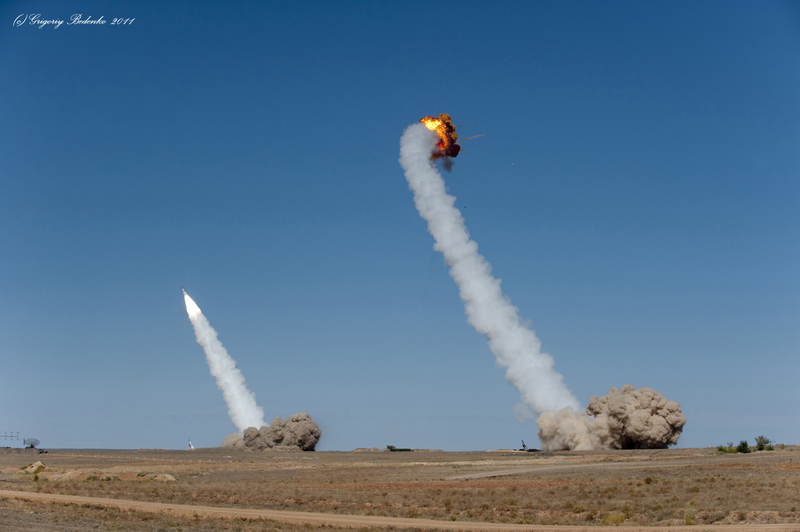
\includegraphics[width=\textwidth]{copy.jpg}
    \end{figure}
}

\frame{
    \frametitle{Live upgrade}
    \begin{figure}[htb]
    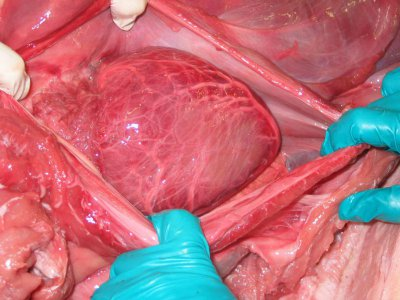
\includegraphics[width=\textwidth]{live.jpg}
    \end{figure}
}

\frame{
    \frametitle{Conclusion}
    \begin{itemize}
    \item automate everything what you can
    \item test new version in production environment
    \item use read-only mode, for drammatic updates
    \end{itemize}
}

\frame{
    \frametitle{Questions and Answers}
    \begin{itemize}
    \item Maksim Melnikau (max\_posedon)
    \item email: m\_melnikau@wargaming.net
    \end{itemize}
}

\end{document}
